\documentclass[tikz]{standalone}

% === GENERAL === (((
\newcommand{\tipoAvaluo}{Maquinaria}
\newcommand{\bienesValuados}{Maquinaria y Equipo para selección y embolsado de nuez}
\newcommand{\objetoValuacion}{Estimar su Valor Razonable y Valor de Liquidación Forzada}
\newcommand{\propositoValuacion}{Identificar posibles sectores agroindustriales para comercializar los equipos para su venta}
\newcommand{\condicionAvaluo}{Desinstalados y fuera de operación}
% )))

% === UBICACIÓN === (((
\newcommand{\calle}{13 Norte}
\newcommand{\numExterior}{1400}
\newcommand{\numInterior}{No aplica}
\newcommand{\colonia}{Terrazas}
\newcommand{\municipio}{Delicias}
\newcommand{\codigoPostal}{33106}
\newcommand{\ciudad}{Delicias}
\newcommand{\entidadFederativa}{Chihuahua}
\newcommand{\direccion}{\calle \numExt, \numInt. \colonia. \municipio \ciudad.
\entidadFederativa. CP \codigoPostal.}
\newcommand{\latitud}{\(28 ^ \circ 13'29.50\)"N}
\newcommand{\longitud}{\(105 ^ \circ 27'28.60\)"O}
\newcommand{\altitud}{\(1,173\) msnm}
\newcommand{\sucursal}{No aplica}
% )))

% === REMITENTES === (((
\newcommand{\personaSolicitante}{María Luisa Alejandra Álvarez Ortega}
\newcommand{\nombrePropietario}{BBVA Leasing México S.A. de C.V.}
% )))

% === FECHA INFORME Y VALORES === (((
\newcommand{\diaInforme}{4 }
\newcommand{\mesInforme}{Septiembre }
\newcommand{\annoInforme}{2024}
\newcommand{\fechaInforme}{\diaInforme de \mesInforme de \annoInforme}
% \newcommand{\fechaInformeCompacta}{\diaInforme/\mesInforme/\annoInforme}

\newcommand{\diaValores}{1 }
\newcommand{\mesValores}{Septiembre }
\newcommand{\annoValores}{2024}
\newcommand{\fechaValores}{\diaValores de \mesValores de \annoValores}
% \newcommand{\fechaValoresCompacta}{\diaValores/\mesValores/\annoValores}

\newcommand{\diaInspeccion}{3 }
\newcommand{\mesInspeccion}{Septiembre }
\newcommand{\annoInspeccion}{2024}
\newcommand{\fechaInspeccion}{\diaInspeccion de \mesInspeccion de \annoInspeccion}
% \newcommand{\fechaInspeccionCompacta}{\diaInspeccion/\mesInspeccion/\annoInspeccion}
% )))

% === PERITO VALUADOR === (((
\newcommand{\peritoValuador}{Diego Miguel Perezcano Beltrán}
\newcommand{\descripcionFirmaPerito}{
	Corredor Público No. 2 de la \\
	Plaza del Estado de México. \\ 
	Especialista en Valuación con orientación en \\ 
	Negocios en Marcha. Cédula SEP 10548258 \\ 
	Maestría: Valuación en Maquinaria y Equipo.
}
\newcommand{\cResponsable}{No aplica}
\newcommand{\cedulaProfesional}{13782921}
% )))

% === VALUACION === (((
\newcommand{\valorMaquinaria}{36,629,000}
\newcommand{\valorMaquinariaLetra}{Treinta y Seis Millones Seiscientos Veintinueve Mil Pesos 00/100 MXN.}
% )))


% === COLORS === (((
\definecolor{principal}{RGB}{0, 53, 73}
\definecolor{secundario}{RGB}{43, 82, 96}
\definecolor{terciario}{RGB}{43,82,96}
% )))

\begin{document}

\begin{tikzpicture}[scale=1.2]

	% === ELEMENTS AROUND THE PAGE === (((
	\clip (-5,-6.6) rectangle (4.95,6.6);
	\node (a) at (0,0) {
\includegraphics[width=  12cm]{../0.imagenes/GENERAL/LOGOS/background_valuami}};
	\fill [white] (-2,-2) rectangle (2,2);
	\node at (0,4.5) {
\includegraphics[width=  4cm,page=1]{../0.imagenes/GENERAL/LOGOS/logo_valuami_fondo_blanco}};
	\node at (3.4,-5) {
\includegraphics[width=  1.5cm]{../0.imagenes/GENERAL/LOGOS/qr}};
	% )))

	% === PARAMETROS=== (((
	\node at (0,-0.5) {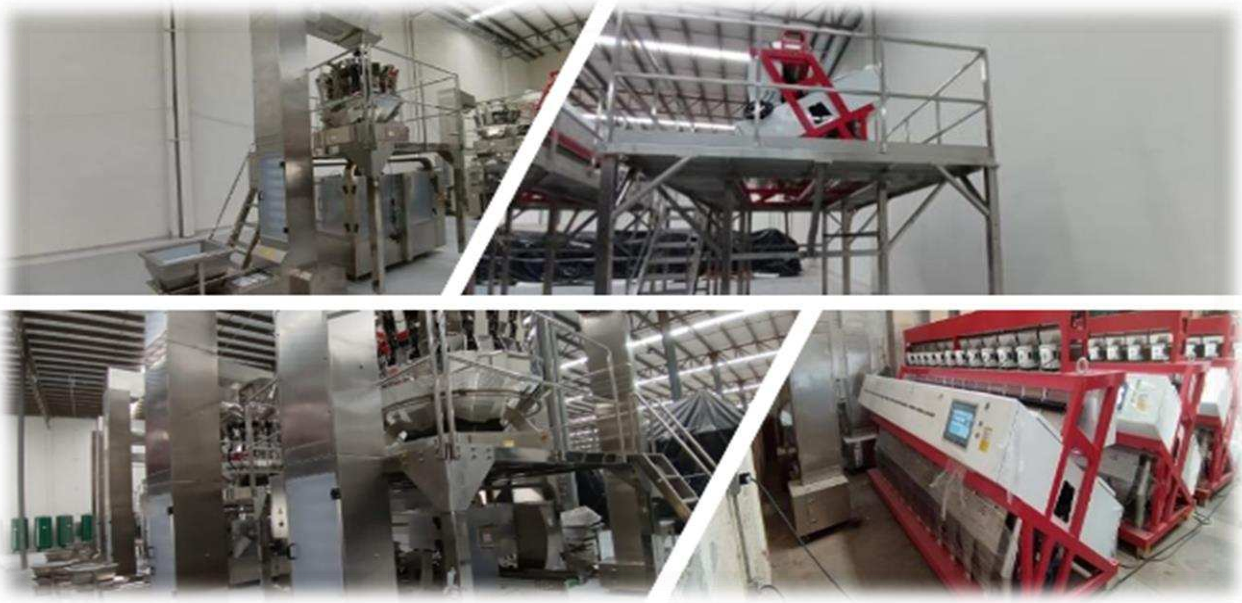
\includegraphics[width= 8cm]{../0.imagenes/PORTADA/1}};
	\node [principal] at (0,2.5) {\shortstack{\sc\Large Valuación de Maquinaria y Equipo \\ \sc para Selección y Embolsado de Nuez.}};
	% )))

	% === DATOS === (((
	\node at (0,-3) {Dictamen de Valuación.};
	\node [black!60,right] at (-4,-4) {\footnotesize Solicitante: \personaSolicitante};
	\node [principal,right] at (-4,-4.5) {\bfseries Mtro. \peritoValuador};
	% \node [right] at (-3,-5) {\footnotesize };
	\node [right] at (-4,-5.3) {\tiny \shortstack[l]{\descripcionFirmaPerito}};
	% )))

	% === GRID FOR DRAWING === (((
	% \draw [help lines] (a.south west) grid (a.north east);
	% \fill [red] (0,0) circle (2pt);
	% )))

\end{tikzpicture}

\end{document}
